%MIT OpenCourseWare: https://ocw.mit.edu
%RES.18-011 Algebra I Student Notes, Fall 2021
%License: Creative Commons BY-NC-SA 
%For information about citing these materials or our Terms of Use, visit: https://ocw.mit.edu/terms.

\section{Orthogonal Matrices}

In this lecture, we start formally studying the symmetry of shapes, combining group theory with linear algebra. The matrices considered will be over $\RR$, the field of real numbers, rather than $\CC$.

\subsection{Dot Products and Orthogonal Matrices}


Recall the following definitions.
\begin{definition}
    Given column vectors $x, y \in \RR^n$, the \textbf{dot product} is defined as $x \cdot y = x^T y = \sum_{i=1}^n x_i y_i$. The \textbf{length} of a vector $v$ is $|v| = \sqrt{v \cdot v}.$
\end{definition}

The dot product is defined algebraically, but also carries geometric information about two vectors: \[x \cdot y = |x||y|\cos\theta.\] Moreover, if $x \cdot y = 0,$ then $x$ and $y$ will be perpendicular vectors in $\RR^n.$

To start out with, consider bases for which the pairwise dot products are as simple as possible.
\begin{definition}
    A basis $\{v_1, \cdots, v_n\}$ is called \emph{orthonormal} if $|v_i| = 1$ and $v_i \cdot v_j = 0$ for $i \neq j.$ That is, since $|v_i| = \sqrt{v_i \cdot v_i},$ \[v_i \cdot v_j = \delta_{ij},\] where $\delta_{ij}$ denotes the Kronecker delta.\footnote{The Kronecker delta $\delta_{ij}$ is equal to 0 if $i \neq j$ and 1 if $i = j.$}
    
    % for all basis vectors $v_i$, $|v_i| = 1$, and if $v_i \cdot v_j = 0$ for $i \neq j$. That is, if $v_i \cdot v_j = $
\end{definition}

Now, $\RR^n$ not only has a vector space structure, but it also has some extra structure provided by the dot product. Since $|v| = \sqrt{v \cdot v}$, the dot product produces some notion of "length" or "distance." 

\begin{qq}
What kinds of matrices interact well with this notion of distance?
\end{qq}

Orthogonal matrices are those preserving the dot product.
\begin{definition}
    A matrix $A \in GL_n(\RR)$ is \emph{orthogonal} if $Av \cdot A w = v \cdot w$ for all vectors $v$ and $w.$
\end{definition}

In particular, taking $v = w$ means that lengths are preserved by orthogonal matrices. There are many equivalent characterizations for orthogonal matrices.
\begin{theorem}
    The following conditions are all equivalent:
    \begin{enumerate}
        \item The matrix $A$ is orthogonal.
        \item For all vectors $v \in \RR^n,$ $|Av| = |v|$. That is, $A$ preserves lengths.
        \item For an $n$-dimensional matrix $A,$ $A^T A = I_n$.
        \item The columns of $A$ form an orthonormal basis.\footnote{Since $A^T$ also satisfies the third condition, this means that the rows of $A$, which are the columns of $A^T,$ will also form an orthonormal basis.}
    \end{enumerate}
\end{theorem}
\begin{proof}
All the conditions will end up equivalent.
\begin{itemize}
    \item Condition (1) implies (2). Because $A$ preserves dot products, $|Av| = \sqrt{Av\cdot Av} = \sqrt{v\cdot v} = |v|,$ and so $A$ also preserves lengths.
    
    \item Condition (2) implies (1) because
    
    % because \[v \cdot w = \frac{1}{2} \left(|v + w|^2 - |v|^2 - |w|^2\right),\] so 
    \begin{align*}
            Av \cdot Aw &= \frac{1}{2} \left(|Av + Aw|^2 - |Av|^2 - |Aw|^2\right)\\
            &= \frac{1}{2} \left(|v + w|^2 - |v|^2 - |w|^2\right) \\
            &= v \cdot w.
    \end{align*} 
    Namely, dot products can be written in terms of lengths, and lengths can be written in terms of dot products, so preserving one is equivalent to preserving the other.

    \item Condition (1) states that $Av \cdot Aw = v \cdot w$; unwinding the dot product in terms of matrix multiplication, this equation is $v^TA^TAw = v^Tw$ for all $v, w \in \RR^n.$ Evidently, (3) implies (1), since if $A^TA = I_n,$ $v^TA^TAw = v^Tw.$ 
    
    By calculation, it can be seen that for $e_i$ and $e_j$ the $i$th and $j$th standard basis vectors, $e_i^T M e_j = M_{ij},$ which is the $(i, j)$th component of the matrix $M.$ If (1) is true, taking $v = e_i$ and $w = e_j$ over all $i$ and $j$ gives us that the $(i, j)$th component of $A^TA$ is 1 when $i = j$ and 0 otherwise.


    \item Condition (4) is equivalent to (3) from simply computing the matrix product: the $(i, j)$th entry of $A^TA$ is the dot product of the $i$th column of $A$ with the $j$th column of $A,$ which is 1 when $i = j$ and 0 otherwise.

\end{itemize}
\end{proof}

Orthogonal matrices preserve lengths, as well as preserving angles up to sign. In general, a set of matrices satisfying some well-behaved properties of a set of matrices generally form a subgroup, and this principle does hold true in the case of orthogonal matrices.
\begin{proposition}
    The orthogonal matrices form a subgroup $O_n$ of $GL_n$. 
\end{proposition}
\begin{proof}
    Using condition (3), if for two orthogonal matrices $A$ and $B,$ $A^TA = B^TB = I_n$, it is clear that $(AB)^TAB = B^TA^TAB = B^TB = I_n$. The other subgroup properties are not difficult to verify. 
\end{proof}

\subsection{The Special Orthogonal Group}

Given an orthogonal matrix $A,$ $A^TA = I_n,$ and so $\det(A^TA) = \det(A^T)\det(A) = \det(A)^2 = \det(I_n) = 1.$ As a result, $\det(A) = \pm 1.$ The determinant is a homomorphism from $\det: GL_n \rto \RR,$ and the restriction to $O_n$ is a homomorphism $\det: O_n \rto \{\pm 1\}.$ The kernel forms a subgroup of $O_n.$

\begin{definition}[Special Orthogonal Group]
The orthogonal matrices with determinant 1 form a subgroup $SO_n \subset O_n \subset GL_n$ called the \textbf{special orthogonal group}.
\end{definition}

Because the determinant is surjective\footnote{For example, the identity matrix is always orthogonal and has determinant 1, and the diagonal matrix with $-1$ in the first row and column and 1 down the rest of the diagonal is also orthogonal and has determinant $-1$.}, the kernel, $SO_n,$ is an index 2 subgroup inside of $O_n.$ The two cosets are $SO_n$ itself and all the matrices with determinant $-1.$

To gain some intuition for orthogonal matrices, we will look at some examples! For $n = 1,$ the orthogonal group has two elements, $[1]$ and $[-1],$ which is not too interesting.

\subsection{Orthogonal Matrices in Two Dimensions}
What are the orthogonal matrices in two dimensions?

\begin{example}[$O_2$]
Describing an element of $O_2$ is equivalent to writing down an orthonormal basis $\{v_1, v_2\}$ of $\RR^2.$ Evidently, $v_1$ must be a unit vector, which can always be described as $v_1 = \begin{pmatrix} \cos\theta \\ \sin\theta \end{pmatrix}$ for some angle $\theta.$ Then $v_2$ must also have length 1 and be perpendicular to $v_1.$ There are two choices, $
v_2 = \begin{pmatrix}
-\sin\theta \\
\cos\theta
\end{pmatrix} \text{ or } \begin{pmatrix}
\sin\theta \\
-\cos\theta
\end{pmatrix}.$ This characterizes all $2\by 2$ orthogonal matrices:
\[
O_2 = \left\{ 
\begin{pmatrix}
\cos \theta  & - \sin \theta \\
\sin \theta & \cos \theta \end{pmatrix}
,\begin{pmatrix}
\cos \theta & \sin \theta \\
\sin \theta & -\cos \theta
\end{pmatrix} 
\right\}.
\]
\begin{center}
    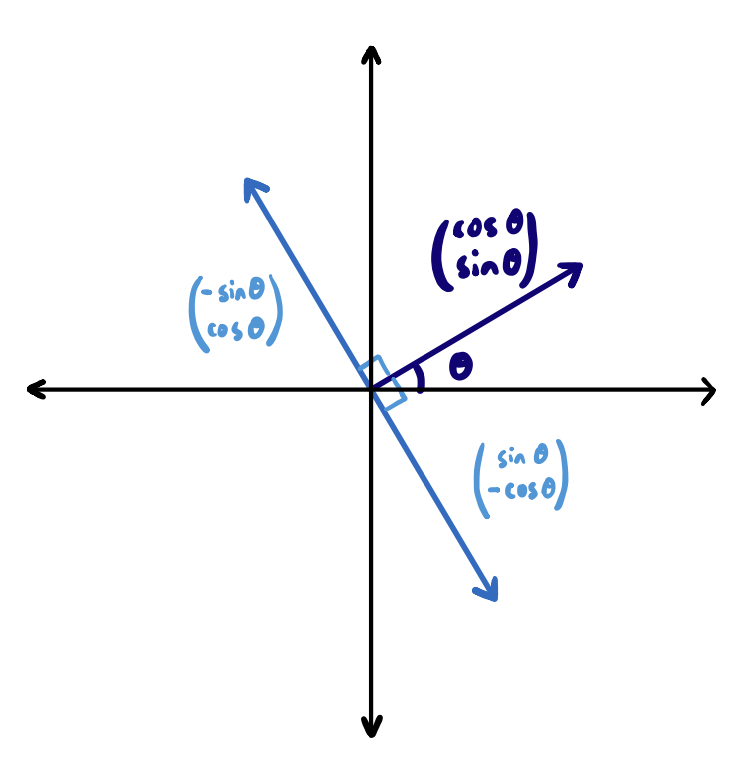
\includegraphics[width=8cm]{Lecture Files and Images/lec12-1.png}
\end{center}
\end{example}


In particular, the first type of matrix has determinant 1, and forms the subgroup $SO_n$, and the second has determinant $-1$ and forms its the non-trivial coset. Geometrically, the first type of matrix in $O_2$ are rotations by $\theta$ around the origin. The matrices of the second type, $A = \begin{pmatrix}
\cos \theta & \sin \theta \\
\sin \theta & -\cos \theta
\end{pmatrix},$ have characteristic polynomial $p_A(t) = t^2 - 1 = (t + 1)(t - 1)$. Thus, they have distinct eigenvalues $\pm 1,$ in contrast to rotation matrices, which do not have any real eigenvalues. Because the eigenvalues are distinct, there is an eigenbasis $\{\vec{v_+}, \vec{v_-}\}$.


\begin{theorem}
    The matrices of the second type are reflections across a line through the origin at an angle of $\theta/2$.
    
    \begin{center}
    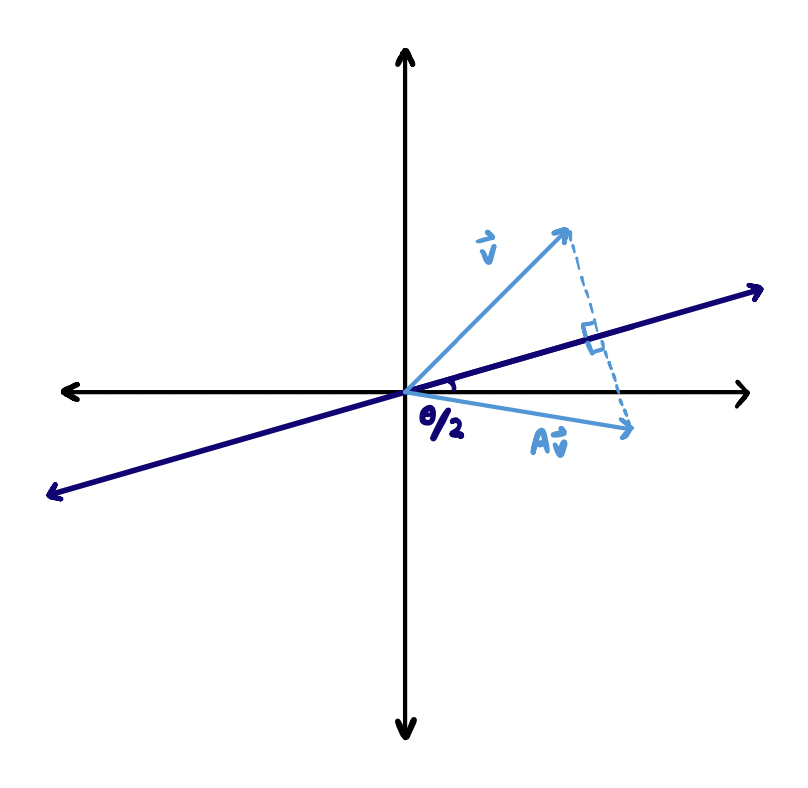
\includegraphics[width=7cm]{Lecture Files and Images/lec12-2.png}
\end{center}
\end{theorem}
\begin{proof}
Consider the line $L = \spann(\vec{v_+});$ since $\vec{v_+}$ is an eigenvector with eigenvalue 1, $A$ fixes this line. Notice that \[\vec{v_+} \cdot \vec{v_-} = A\vec{v_+} \cdot A \vec{v_-} = \vec{v_+} \cdot (-\vec{v_-}),\] where the first equality comes from the fact that $A$ is orthogonal, and the second comes from the eigenvalues $1$ and $-1$ of $v_+$ and $v_-$. The only possibility is $\vec{v_+} \cdot \vec{v_-}  = 0,$ so the two eigenvectors are orthogonal. Writing out any other vector in terms of the eigenvectors, $Av$ is precisely the reflection across $L$. 

\begin{center}
    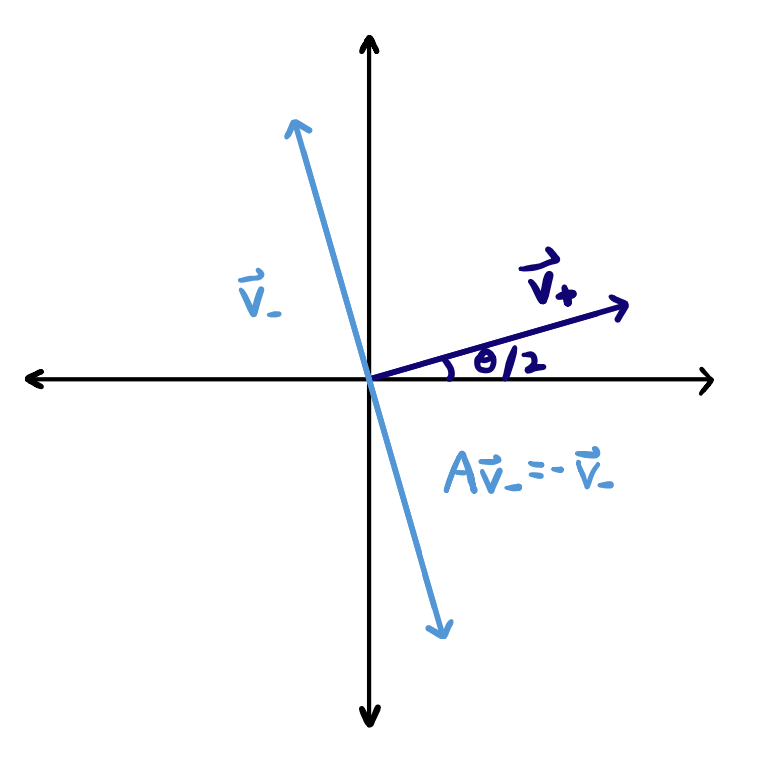
\includegraphics[width=7cm]{Lecture Files and Images/lec12-3.png}
\end{center}

\end{proof}

As expected, rotations and reflections preserve distance, and in fact they make up all the $2 \by 2$ orthogonal matrices. A fun fact that comes from this analysis is that the composition of two reflections over different lines will be a rotation, since the product of determinants will be $(-1)\cdot(-1) = 1.$ Orthogonal matrices can be thought of either geometrically or algebraically!

\subsection{Orthogonal Matrices in Three Dimensions}


In two dimensions, $SO_2$ consists of rotation matrices. It turns out that in three dimensions, $SO_3$ also consists of rotation matrices. 

In particular, a rotation in $\RR^3$ is characterized by the axis of the rotation, which is a unit vector $\vec{u} \in \RR^3$, and the angle of the rotation, which is some $\theta \in \RR.$
The plane \[u^{\perp} = \{v \in \RR^3: u \cdot v = 0\}\] consists of all the vectors in $\RR^3$ that are perpendicular to $\RR^3.$ 

\begin{center}
    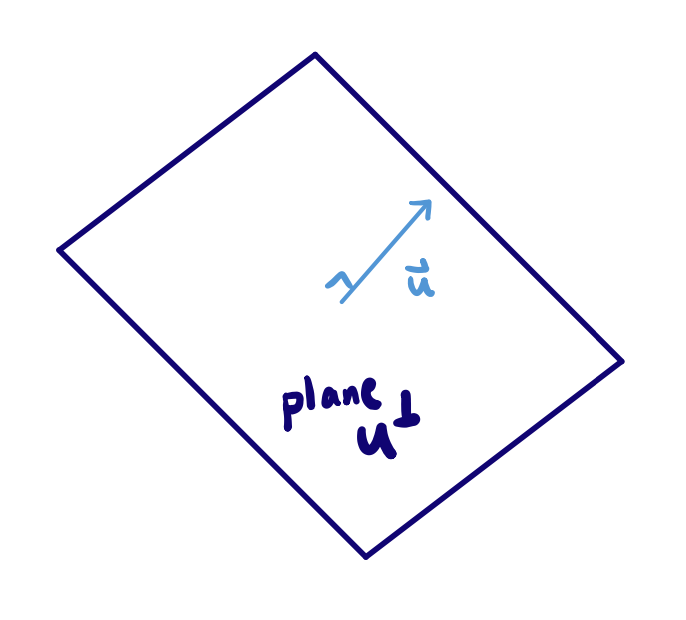
\includegraphics[width=7cm]{Lecture Files and Images/lec12-4.png}
\end{center}

\begin{definition}
The \textbf{rotation operator} with \textbf{spin labels} $u$ and $\theta$ is $\rho_{(u, \theta)},$ the linear operator $\rho: \RR^3 \rto \RR^3$ such that $\rho(u) = u$ and $\rho|_{u^{\perp}}$ is the rotation by $\theta$ counterclockwise with respect to the direction that $u$ points in.\footnote{Since every vector in $\RR^3$ is a linear combination of $u$ and some vector in $u^{\perp},$ the rotation operator is described completely by these conditions.}
\end{definition}

There is some redundancy in this description; for example, $\rho_{(u, \theta)} = \rho_{(-u, -\theta)}.$
\begin{theorem}
The rotation operators are exactly $SO_3$.
\end{theorem}
From geometric intuition, this result is not very surprising, since rotations preserve distance.\footnote{And orientation}
\begin{proof}

First, we show that all the rotation matrices are in $SO_3,$ and then we show that all matrices in $SO_3$ are rotation matrices.
\begin{itemize}
    \item  We first show that all of these rotation matrices belong to $SO_3$. Let $\{v, w\}$ be an orthonormal basis for the plane $u^\perp$, and let $P$ be a $3\times 3$ matrix with columns $(u,v,w)$. Since $v$ and $w$ are orthogonal to each other, and $u$ is orthogonal to both $v$ and $w,$ $P \in O_3.$ Conjugating a rotation matrix by $P$ demonstrates the action of $\rho_{(u, \theta)}$ with respect to the basis $(u, v, w).$ Since $u$ is fixed by the rotation matrix, the first column is $(1, 0, 0)^t,$ and since the plane $u^{\perp}$ is being rotated by $\theta,$ the rest of the matrix $M$ is given by the form of a $2 \by 2$ rotation matrix. That is,
    \[
    P^{-1}\rho_{(u, \theta)}P = \begin{pmatrix} 1 & 0 & 0 \\ 0 & \cos \theta & -\sin \theta \\ 0 & \sin \theta & \cos \theta \end{pmatrix} = M,
    \] which is in $SO_3.$ Since $\rho_{(u, \theta)} = PMP^{-1},$ and since $P, P^{-1} \in O_3$ and $M \in SO_3,$ the rotation matrix $\rho_{(u, \theta)}$ is also in $O_3.$ Taking the determinant of both sides\footnote{$\det(PMP^{-1}) = \det(P)\det(M)\det(P)^{-1} = \det(M) = 1$} demonstrates that $\rho_{(u, \theta)} \in SO_3.$
    
\item 
    To show the other direction, an element $A \in SO_3$ must be shown to be rotation around some axis $u,$ which has to be some eigenvector with eigenvalue $\lambda = 1$. There exists such an eigenvector if and only if $1$ is a root of the characteristic polynomial of $A,$ which is precisely when $\det(I-A) = 0.$
    
    Since $\det(A^T) = 1,$ $\det(A - I) = \det(A^T(A - I)).$ Using the fact that $A$ is orthogonal, this is $\det(I - A^T).$ Taking the transpose, this is $\det(I - A).$ Since the matrices are $3 \by 3,$ $\det(I-A) = (-1)^3\det(A-I).$
    Combining these,
    \begin{align*}
        \det(A-I) &= \det(A^T (A - I)) \\
                  &= \det(I - A^T) \\
                  &= \det(I-A) \\
                  &= (-1)^3 \det(A-I),
    \end{align*}
    implying that $\det(A-I) = 0.$ Therefore, there does exist an eigenvector of eigenvalue 1 for $A,$ which can be scaled to be a unit vector $u.$

    We extend $u$ to an orthonormal basis $P = (u, v, w)$ by picking an orthonormal basis for $u^\perp$. Consider taking $A$ in this basis. The first column is $(1, 0, 0)^t$, since $u$ is an eigenvector, and the first row is $(1, 0, 0)$ because the columns are orthogonal. Then, the bottom right submatrix is an element of $SO_2$ by taking the determinant. 
    So \[P^{-1} AP =
    \begin{pmatrix}
        1 & 0 & 0 \\
        0 & \cos & -\sin \\
        0 & \sin & \cos
    \end{pmatrix},
    \]
    and we are done.
\end{itemize}

\end{proof}

\newpage